\documentclass{article}
\usepackage[polish]{babel}
\usepackage{minted}
\usepackage[letterpaper,top=2cm,bottom=2cm,left=3cm,right=3cm,marginparwidth=1.75cm]{geometry}
\usepackage{amsmath}
\usepackage{graphicx}
\usepackage[colorlinks=true, allcolors=blue]{hyperref}
\usepackage[T1]{fontenc}
\usepackage[table,xcdraw]{xcolor}
\usepackage{float}
\usepackage[figurename=Wykres]{caption}
\usepackage{amsmath}

\title{MOwNiT - Aproksymacja trygonometryczna}
\author{Jakub Frączek}

\begin{document}

\maketitle

\section{Funkcja dla której przeprowadzone zostało doświadczenie}

\begin{center}
\(f(x) = 10 * m + \frac{\mathrm{x}_{}^{2}}{k} - 10 * m * cos(k*x)\)
\end{center}

\noindent
gdzie:

\bigbreak

\(k = 1.5\)
\newline \indent
\(m = 3.0\)
\newline \indent
\(x \in [-4\pi, 4\pi]\)

\bigbreak

\noindent
Wykres funkcji:

\begin{figure}[H]
  \centering
  \begin{minipage}[b]{0.5\textwidth}
    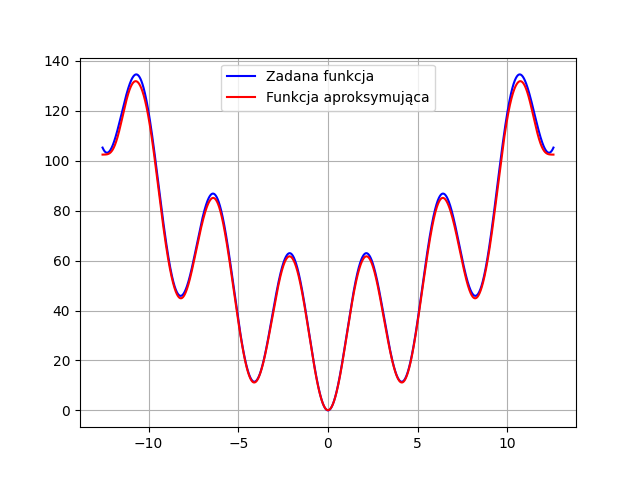
\includegraphics[width=\textwidth]{zadana_funkcja.png}
  \end{minipage}
\end{figure}

\section{Dane techniczne}

\subsection{Hardware}

Laptop z procesorem Intel Core i5-9300H 2.4GHz oraz 32 GB pamięci RAM.

\subsection{Software}

Wykorzystany został system Windows 11 x64 oraz język Python w wersji 3.11.8 wraz z bibliotekami:
\begin{itemize}
\item math
\item copy
\item matplotlib
\item numpy
\end{itemize}

\newpage

\section{Aproksymacja}

Ogólny wzór na przybliżenie aproksymacyjne

\[F(x) = c_o\phi_o(x) + c_1\phi_1(x) + ... + c_m\phi_m(x) = \Sigma_{i=0}^{m}c_i\phi_i(x)\]

\noindent
W tym przypadku za funkcje bazowy przyjmuję
\[(\phi_i(x)) = 1, sin(x), cos(x), sin(2x), cos(2x), ..., sin(mx), cos(mx)\]

\noindent
Wzory przybliżające szukaną funkcję wielomianem trygonometrycznym

\[F_m(x) = \frac{1}{2} \cdot a_0 + \Sigma_{j=1}^{m}(a_j \cdot cos(j \cdot x) + b_j \cdot sin(j \cdot x)\]

\[a_j = \frac{2}{n} \cdot \Sigma_{i=0}^{n-1}f(x_i) \cdot cos(j \cdot x_i)\]

\[b_j = \frac{2}{n} \cdot \Sigma_{i=0}^{n-1}f(x_i) \cdot sin(j \cdot x_i)\]

\noindent
Przyjmując n + 1 rónoodległych węzłów aproksymacji opisanych wzorem \(x_i = n \cdot i \cdot \frac{\pi}{2}\), to kolejne elementy bazy będą do siebie ortogonalne i stworzą układ normalny dobrze uwarunkowany.

\noindent
Wielomianami trygonometrycznimi można aproksymować dowolną funkcję okresową, jak wynika z tw. Weierstrassa

\bigbreak

\noindent
Tw. Weierstrassa: Jeśli \( f(x) \) jest funkcją określoną i ciągłą w przedziale \( [a, b] \) oraz okresową o okresie równym \( 2\pi \) i dane jest \( \epsilon > 0 \), to wówczas istnieje wielomian trygonometryczny \( W(x) \), określony w \( [a, b] \) taki, że \( |f(x) - W(x)| < \epsilon \) dla każdego \( x \in [a, b] \).

\section{Metody szacowania błędu przybliżenia funkcji}

Wszystkie błędy zostały policzone z dokładnością do 100 równoodległych punktów.

\subsection{Największa różnica wartości funkcji}

Największa różnica między wartością funkcji aproksymowanej, a funkcji aproksymującej:

\begin{center}
    \(\max_{x\in [a, b]} |F(x) - \mathrm{P}_{n}^{}(x)|\)
\end{center}

\subsection{Błąd średniokwadratowy}

Suma kwadratów różnic mięcy wartością funkcji aproksymowanej, a funkcji aproksymującej podzielona przez liczba punktów, w których wykonujemy porównanie:

\begin{center}
\(\frac{1}{N} * \sum_{i = 1}^{N}\mathrm{(F(\mathrm{x}_{i}^{}) - \mathrm{P}_{n}^{}(\mathrm{x}_{i}^{}))}_{}^{2}\)
\end{center}

\section{Analiza}

Podczas analizy funkcji aproksymującej, stopnie wielomianu dobrałem tak, aby nie przekraczały połowy liczby węzłów, co zagwarantowało, że układ był dobrze uwarunkowany.
\noindent
Ilość punktów wykorzystywanych przy liczdeniu błędów średniokwadratowego i maksymalnego oraz rysowaniu funkcji wynosi 1000.

\newpage

\section{Przebieg funkcji dla wybranej liczby węzłów}

\subsection{Dla 6 węzłów}

\noindent
Jak widać na poniższych wykresach (wykres 1, wykres 2), dla 6 węzłów przybliżenie jest bardzo słabe.

\begin{figure}[H]
  \begin{minipage}[b]{0.49\textwidth}
    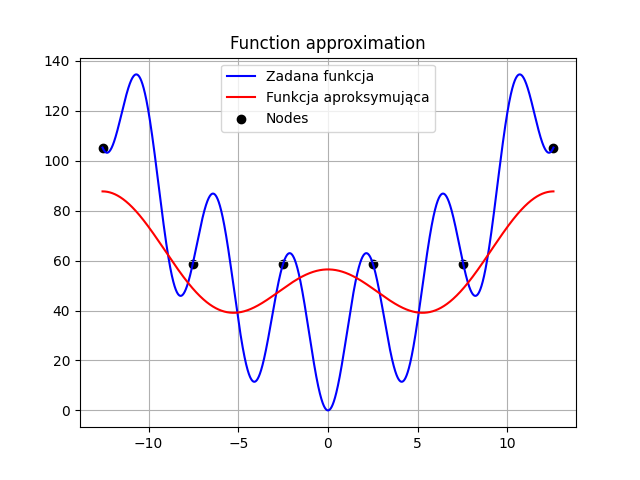
\includegraphics[width=\textwidth]{img01.png}
    \caption{Wielomian 2 stopnia}
  \end{minipage}
  \hfill
  \begin{minipage}[b]{0.49\textwidth}
    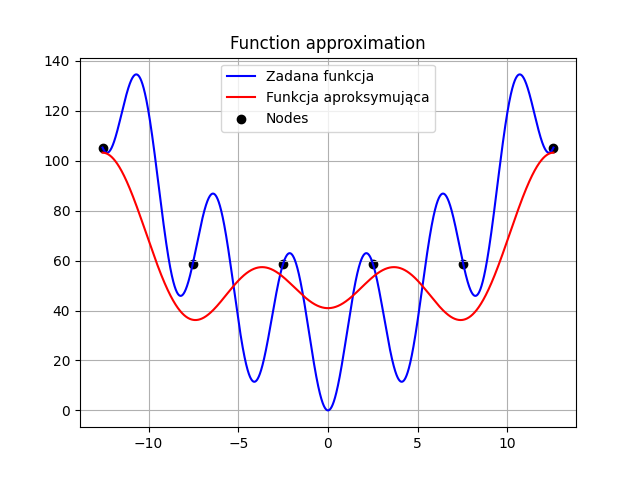
\includegraphics[width=\textwidth]{img02.png}
    \caption{Wielomian 3 stopnia}
  \end{minipage}
\end{figure}

\noindent
Poniżej, na wykresie 3 przedstawione zostały wartości błędów dla wszystkich możliwych stopni wielomianu.

\begin{figure}[H]
  \centering
  \begin{minipage}[b]{0.4\textwidth}
    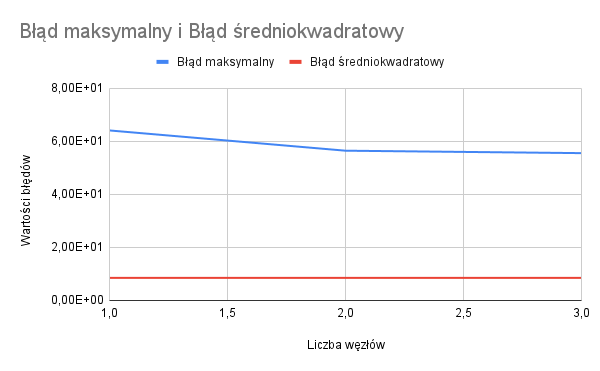
\includegraphics[width=\textwidth]{img03.png}
    \caption{Wartości błędów}
  \end{minipage}
\end{figure}

\newpage

\subsection{Dla 10 węzłów}

\noindent

Dla 10 węzłów aproksymacja jest zuważalnie lepsza, a funkcja aproksymująca zaczyna się lepiej dopasowywać. Niestety zwiększanie stopnia wielomianu powyżej 3 ma niewielki wpływ na dokładność (wykres 4, wykres 5, wykres 5, wykres 6).

\begin{figure}[H]
  \begin{minipage}[b]{0.49\textwidth}
    \begin{minipage}[b]{\textwidth}
      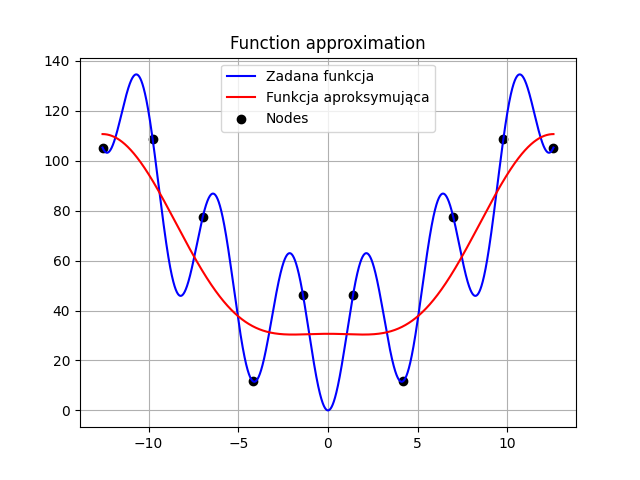
\includegraphics[width=\textwidth]{img04.png}
      \caption{Wielomian 2 stopnia}
    \end{minipage}
    \vspace*{\fill}
    \begin{minipage}[b]{\textwidth}
      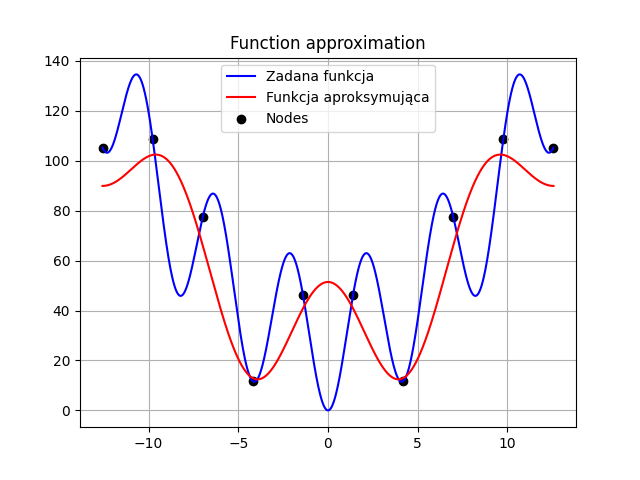
\includegraphics[width=\textwidth]{img05.png}
      \caption{Wielomian 3 stopnia}
    \end{minipage}
  \end{minipage}
  \hfill
  \begin{minipage}[b]{0.49\textwidth}
    \begin{minipage}[b]{\textwidth}
      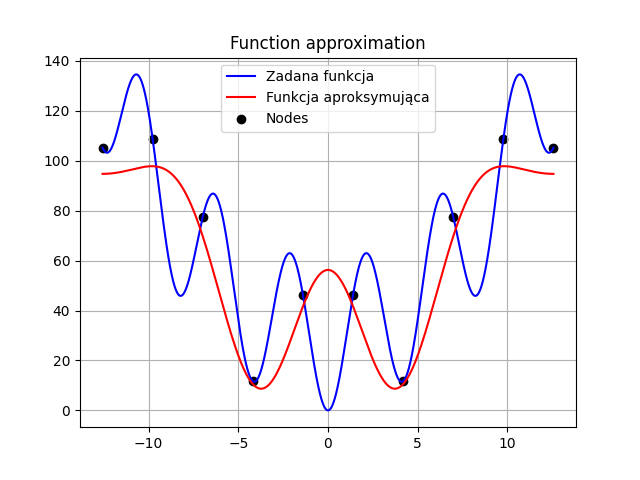
\includegraphics[width=\textwidth]{img06.png}
      \caption{Wielomian 4 stopnia}
    \end{minipage}
    \vspace*{\fill}
    \begin{minipage}[b]{\textwidth}
      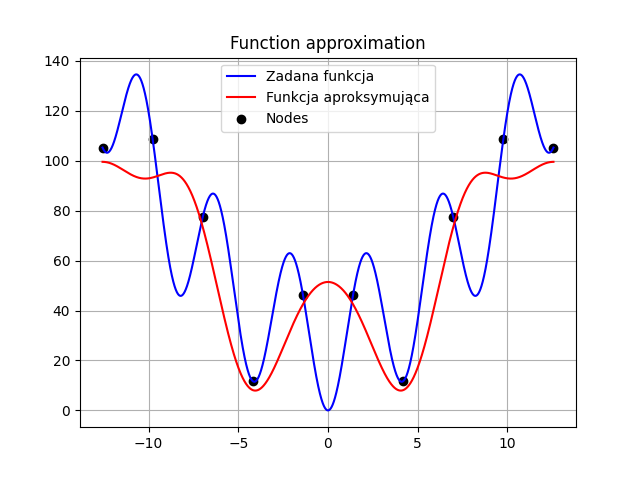
\includegraphics[width=\textwidth]{img07.png}
      \caption{Wielomian 5 stopnia}
    \end{minipage}
  \end{minipage}
\end{figure}

\noindent
Poniżej, na wykresie 8 przedstawione zostały wartości błędów dla wszystkich możliwych stopni wielomianu.

\begin{figure}[H]
  \centering
  \begin{minipage}[b]{0.4\textwidth}
    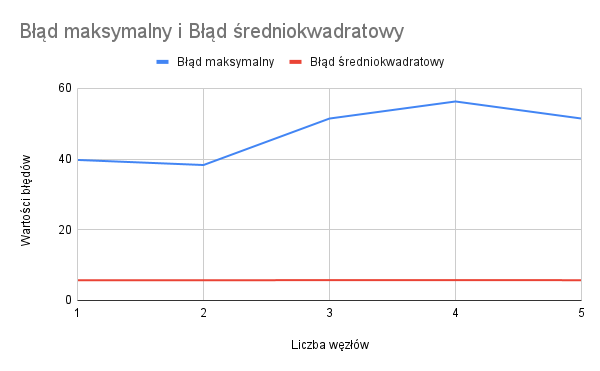
\includegraphics[width=\textwidth]{img08.png}
    \caption{Wartości błędów}
  \end{minipage}
\end{figure}

\newpage

\subsection{Dla 15 węzłów}

\noindent
W tym przypadku od 6 stopnia wielomianu dostajemy całkiem dobre przybliżenie. Jak widać zachodzi znaczna różnica pomiędzy wielomianem stopnia 5 i stopnia 6 (wykres 9, wykres 10, wykres 11 oraz wykres 12).

\begin{figure}[H]
  \begin{minipage}[b]{0.49\textwidth}
    \begin{minipage}[b]{\textwidth}
      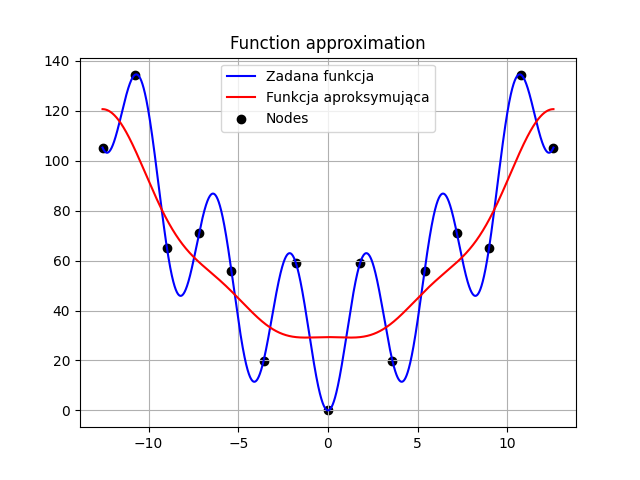
\includegraphics[width=\textwidth]{img09.png}
      \caption{Wielomian 4 stopnia}
    \end{minipage}
    \vspace*{\fill}
    \begin{minipage}[b]{\textwidth}
      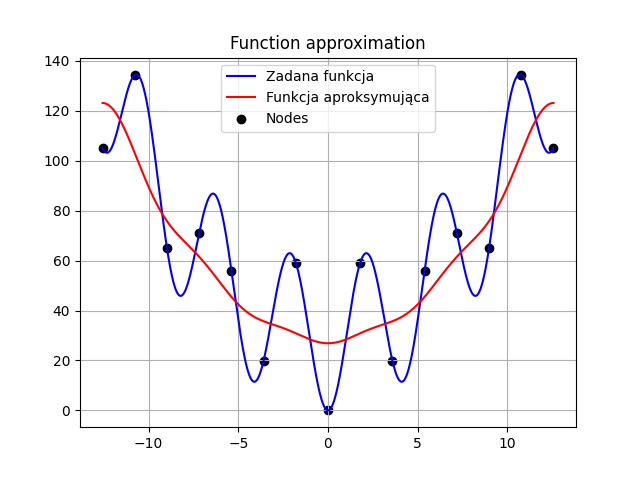
\includegraphics[width=\textwidth]{img10.png}
      \caption{Wielomian 5 stopnia}
    \end{minipage}
  \end{minipage}
  \hfill
  \begin{minipage}[b]{0.49\textwidth}
    \begin{minipage}[b]{\textwidth}
      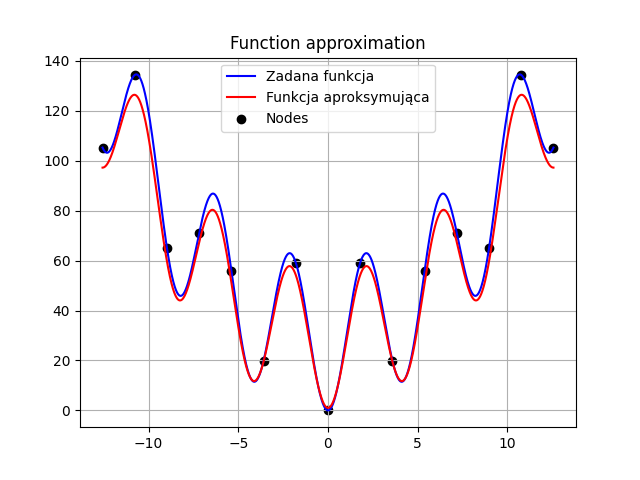
\includegraphics[width=\textwidth]{img11.png}
      \caption{Wielomian 6 stopnia}
    \end{minipage}
    \vspace*{\fill}
    \begin{minipage}[b]{\textwidth}
      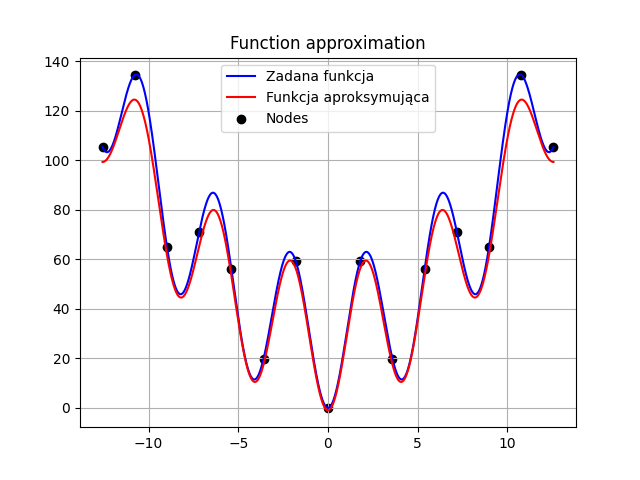
\includegraphics[width=\textwidth]{img12.png}
      \caption{Wielomian 7 stopnia}
    \end{minipage}
  \end{minipage}
\end{figure}

\noindent
Poniżej, na wykresie 13 przedstawione zostały wartości błędów dla wszystkich możliwych stopni wielomianu.

\begin{figure}[H]
  \centering
  \begin{minipage}[b]{0.4\textwidth}
    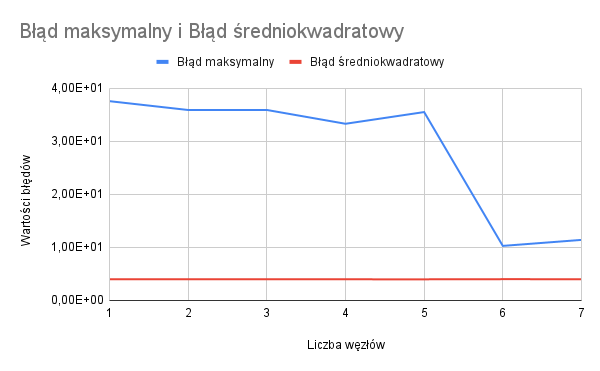
\includegraphics[width=\textwidth]{img13.png}
    \caption{Wartości błędów}
  \end{minipage}
\end{figure}

\newpage

\subsection{Dla 20 węzłów}

\noindent
Tutaj (wykres 14, wykres 15, wykres 16 i wykres 17) przybliżenie jest jeszcze lepsze. Jedynie można zauważyć niedokładność na krańcach przedziału.

\begin{figure}[H]
  \begin{minipage}[b]{0.49\textwidth}
    \begin{minipage}[b]{\textwidth}
      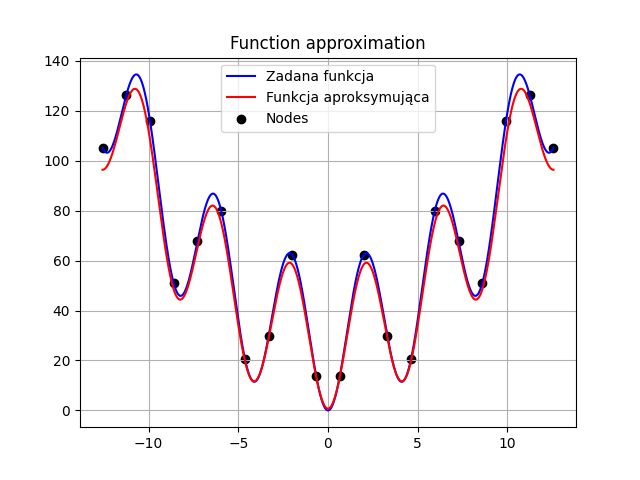
\includegraphics[width=\textwidth]{img14.png}
      \caption{Wielomian 6 stopnia}
    \end{minipage}
    \vspace*{\fill}
    \begin{minipage}[b]{\textwidth}
      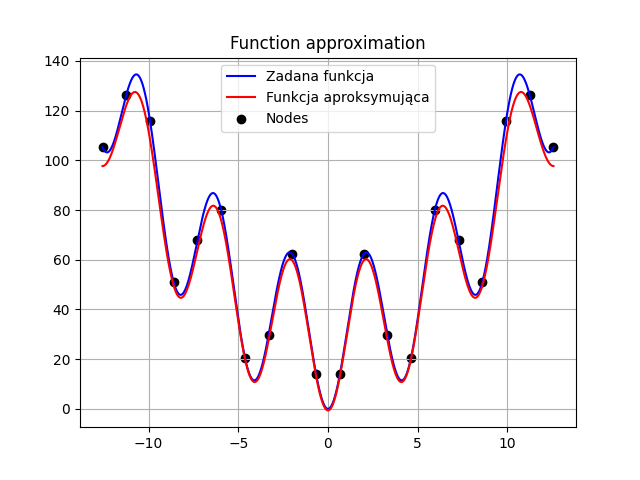
\includegraphics[width=\textwidth]{img15.png}
      \caption{Wielomian 7 stopnia}
    \end{minipage}
  \end{minipage}
  \hfill
  \begin{minipage}[b]{0.49\textwidth}
    \begin{minipage}[b]{\textwidth}
      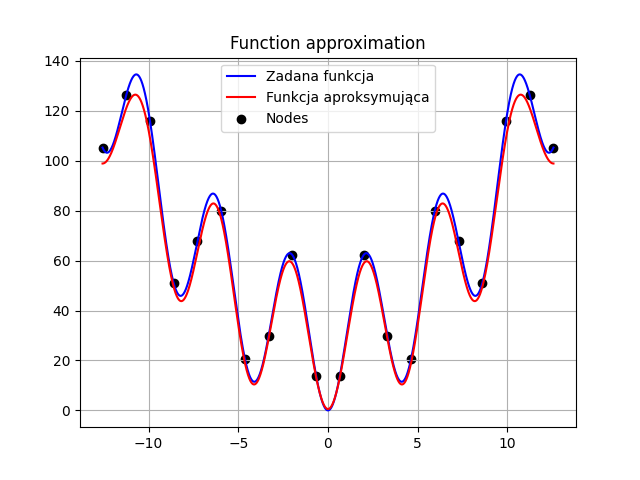
\includegraphics[width=\textwidth]{img16.png}
      \caption{Wielomian 8 stopnia}
    \end{minipage}
    \vspace*{\fill}
    \begin{minipage}[b]{\textwidth}
      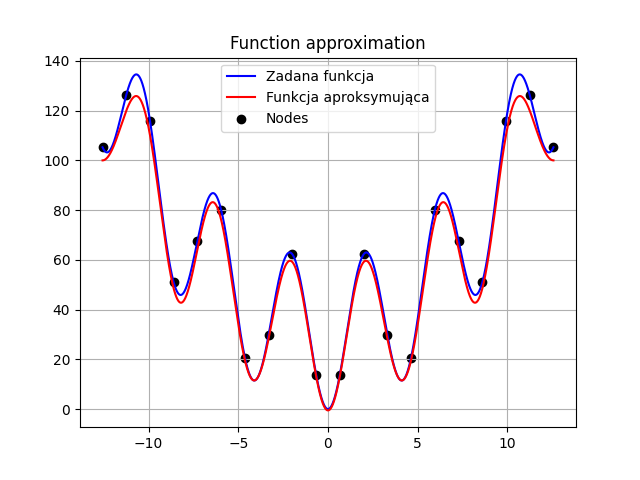
\includegraphics[width=\textwidth]{img17.png}
      \caption{Wielomian 9 stopnia}
    \end{minipage}
  \end{minipage}
\end{figure}

\noindent
Poniżej, na wykresie 18 przedstawione zostały wartości błędów dla wszystkich możliwych stopni wielomianu.

\begin{figure}[H]
  \centering
  \begin{minipage}[b]{0.4\textwidth}
    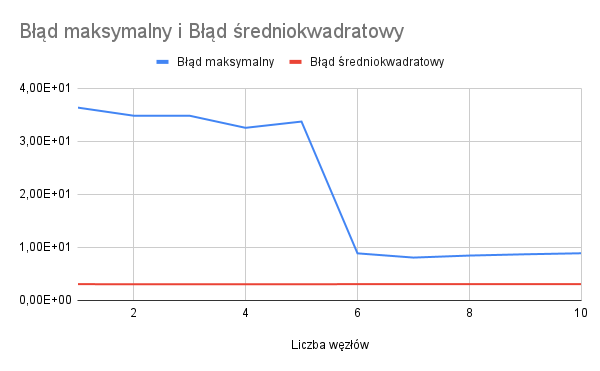
\includegraphics[width=\textwidth]{img18.png}
    \caption{Wartości błędów}
  \end{minipage}
\end{figure}

\newpage

\subsection{Dla 25 węzłów}

\noindent
Jak widać na poniższych wykresach (wykres 19, wykres 20, wykres 21 i wykres 22) przybliżenie jest już dość dobre i pozostaje mniej więcej takie samo dla liczby stopni większej lub równej 6.

\begin{figure}[H]
  \begin{minipage}[b]{0.49\textwidth}
    \begin{minipage}[b]{\textwidth}
      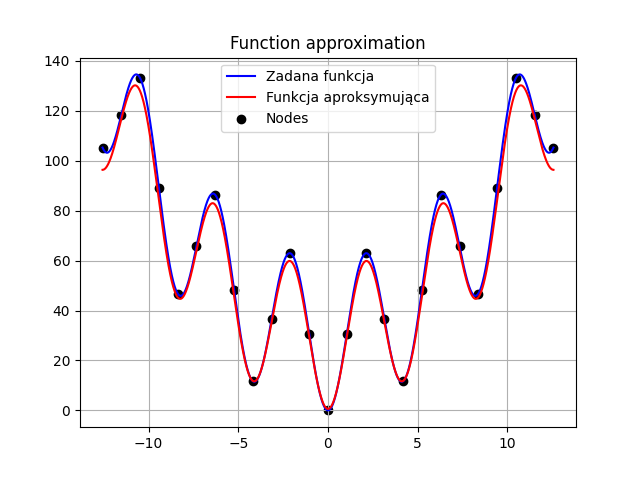
\includegraphics[width=\textwidth]{img19.png}
      \caption{Wielomian 6 stopnia}
    \end{minipage}
    \vspace*{\fill}
    \begin{minipage}[b]{\textwidth}
      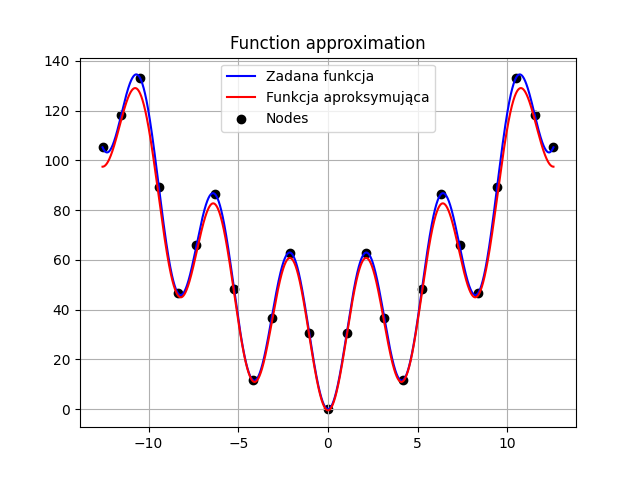
\includegraphics[width=\textwidth]{img20.png}
      \caption{Wielomian 7 stopnia}
    \end{minipage}
  \end{minipage}
  \hfill
  \begin{minipage}[b]{0.49\textwidth}
    \begin{minipage}[b]{\textwidth}
      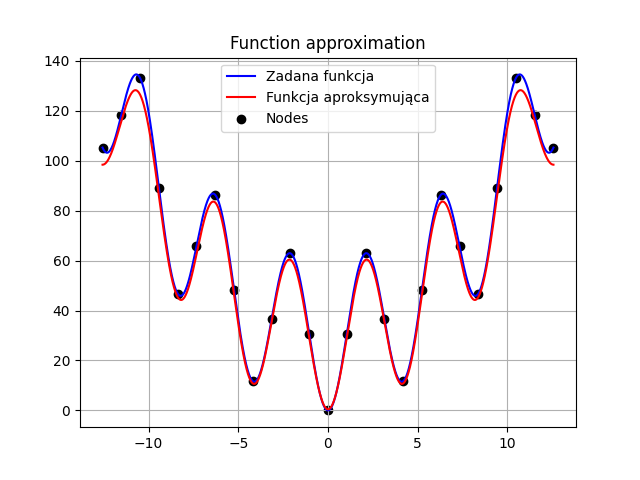
\includegraphics[width=\textwidth]{img21.png}
      \caption{Wielomian 8 stopnia}
    \end{minipage}
    \vspace*{\fill}
    \begin{minipage}[b]{\textwidth}
      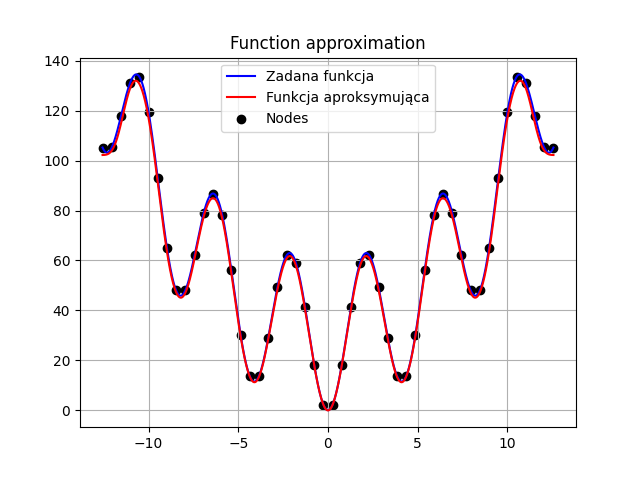
\includegraphics[width=\textwidth]{img22.png}
      \caption{Wielomian 9 stopnia}
    \end{minipage}
  \end{minipage}
\end{figure}

\noindent
Poniżej, na wykresie 23 przedstawione zostały wartości błędów dla wszystkich możliwych stopni wielomianu.

\begin{figure}[H]
  \centering
  \begin{minipage}[b]{0.4\textwidth}
    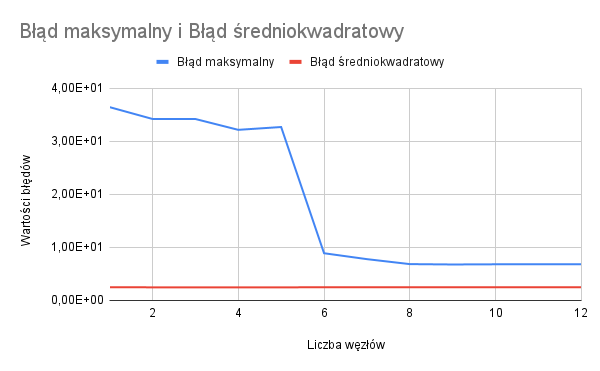
\includegraphics[width=\textwidth]{img23.png}
    \caption{Wartości błędów}
  \end{minipage}
\end{figure}

\newpage

\subsection{Dla 50 węzłów}

\noindent
Dla 50 węzłów przybliżenie jest już bardzo dobre, nie widać błędów na krańcach przedziałów (wykres 24, wykres 25, wykres 26 i wykres 27).

\begin{figure}[H]
  \begin{minipage}[b]{0.49\textwidth}
    \begin{minipage}[b]{\textwidth}
      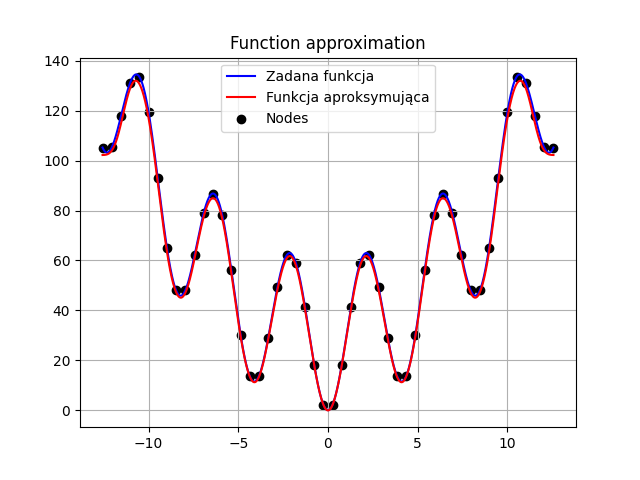
\includegraphics[width=\textwidth]{img24.png}
      \caption{Wielomian 6 stopnia}
    \end{minipage}
    \vspace*{\fill}
    \begin{minipage}[b]{\textwidth}
      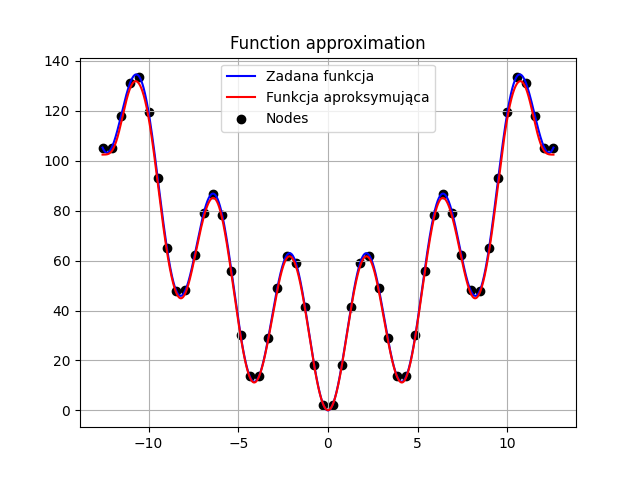
\includegraphics[width=\textwidth]{img25.png}
      \caption{Wielomian 7 stopnia}
    \end{minipage}
  \end{minipage}
  \hfill
  \begin{minipage}[b]{0.49\textwidth}
    \begin{minipage}[b]{\textwidth}
      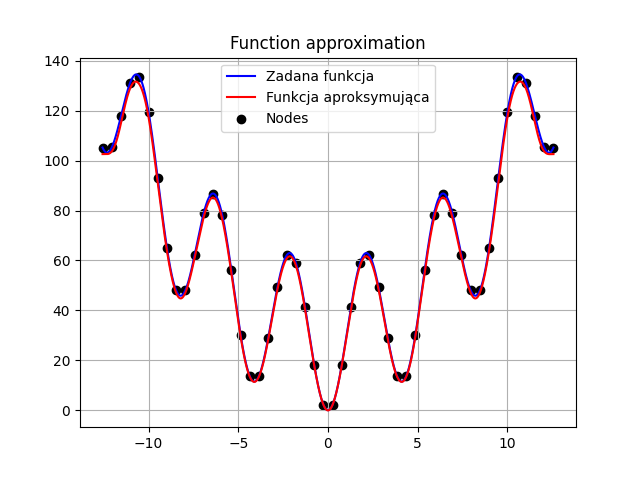
\includegraphics[width=\textwidth]{img26.png}
      \caption{Wielomian 8 stopnia}
    \end{minipage}
    \vspace*{\fill}
    \begin{minipage}[b]{\textwidth}
      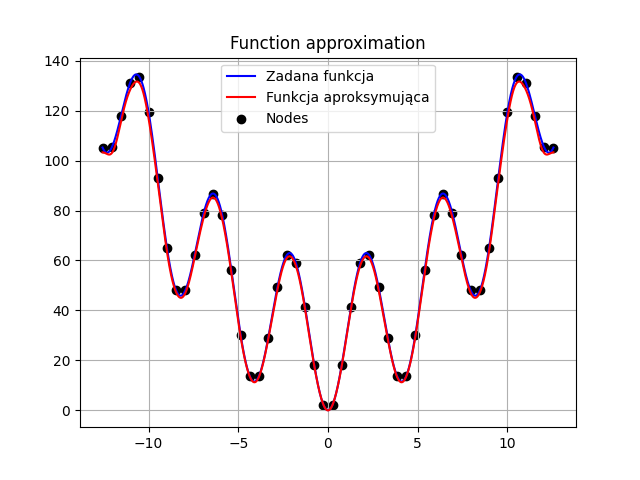
\includegraphics[width=\textwidth]{img27.png}
      \caption{Wielomian 9 stopnia}
    \end{minipage}
  \end{minipage}
\end{figure}

\noindent
Poniżej, na wykresie 28 przedstawione zostały wartości błędów dla wszystkich możliwych stopni wielomianu.

\begin{figure}[H]
  \centering
  \begin{minipage}[b]{0.4\textwidth}
    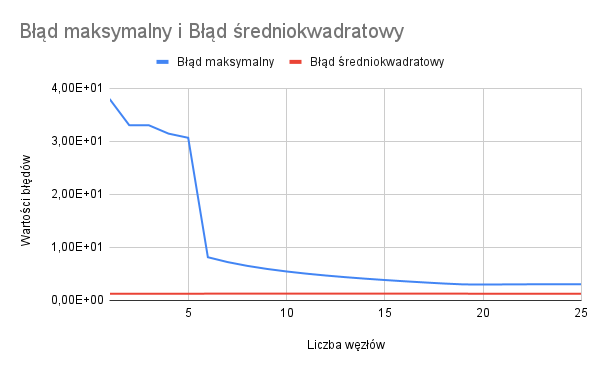
\includegraphics[width=\textwidth]{img28.png}
    \caption{Wartości błędów}
  \end{minipage}
\end{figure}

\newpage

\section{Przebieg funkcji dla wybranego stopnia wielomianu}

\subsection{Dla 5 stopnia}

\noindent
Jak widać na poniższych wykresach (wykres 29, wykres 30, wykres 31 i wykres 32), dla wielomianu 5 stopnia przybliżenie jest złe i zwiększanie liczby węzłów praktycznie nie ma wpływu na dokładność aproksymacji.

\begin{figure}[H]
  \begin{minipage}[b]{0.49\textwidth}
    \begin{minipage}[b]{\textwidth}
      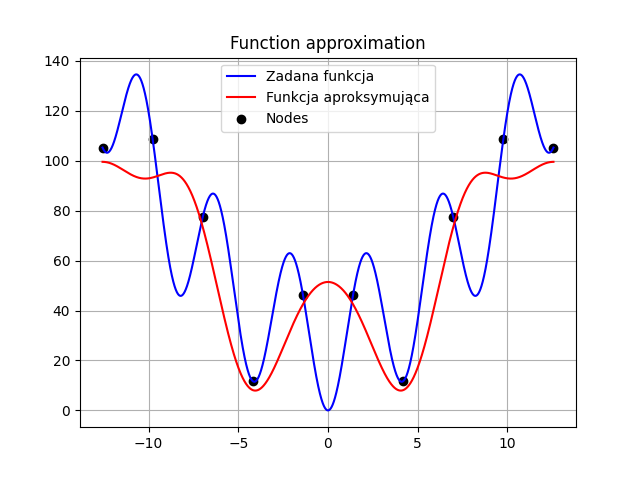
\includegraphics[width=\textwidth]{img29.png}
      \caption{Dla 10 węzłów}
    \end{minipage}
    \vspace*{\fill}
    \begin{minipage}[b]{\textwidth}
      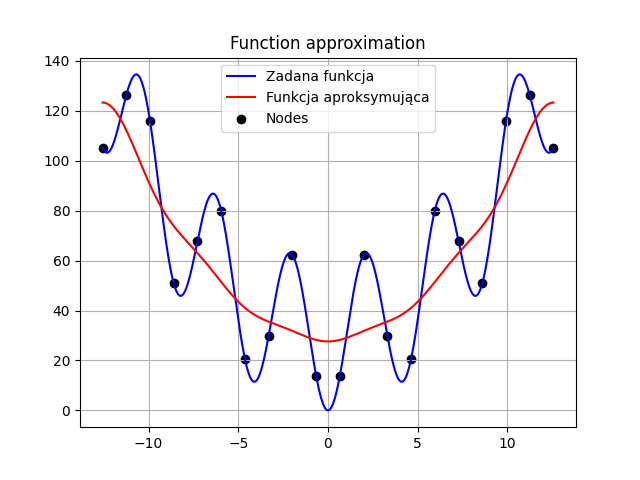
\includegraphics[width=\textwidth]{img30.png}
      \caption{Dla 20 węzłów}
    \end{minipage}
  \end{minipage}
  \hfill
  \begin{minipage}[b]{0.49\textwidth}
    \begin{minipage}[b]{\textwidth}
      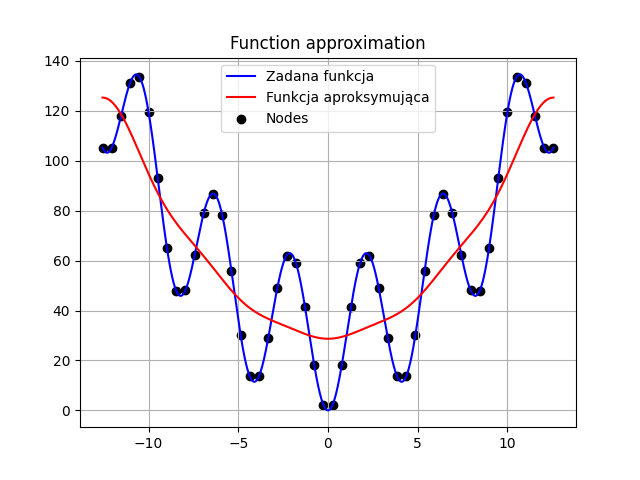
\includegraphics[width=\textwidth]{img31.png}
      \caption{Dla 50 węzłów}
    \end{minipage}
    \vspace*{\fill}
    \begin{minipage}[b]{\textwidth}
      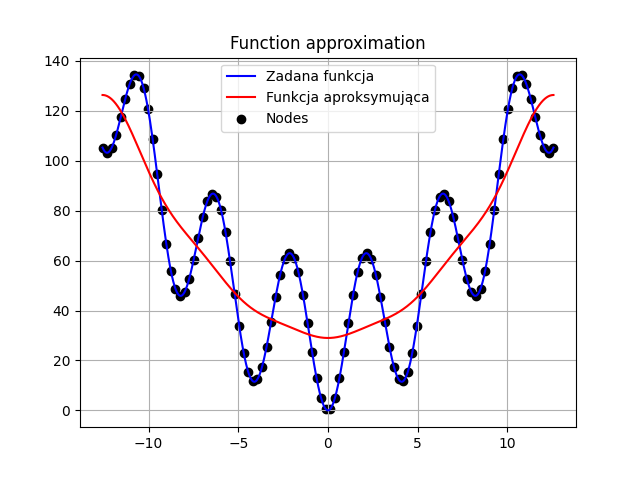
\includegraphics[width=\textwidth]{img32.png}
      \caption{Dla 100 węzłów}
    \end{minipage}
  \end{minipage}
\end{figure}

\noindent
Poniżej, na wykresie 33 przedstawione zostały wartości błędów dla wszystkich możliwych stopni wielomianu.

\begin{figure}[H]
  \centering
  \begin{minipage}[b]{0.4\textwidth}
    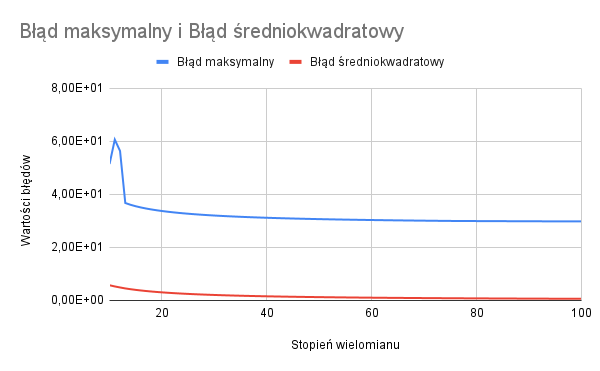
\includegraphics[width=\textwidth]{img33.png}
    \caption{Wartości błędów}
  \end{minipage}
\end{figure}

\newpage

\subsection{Dla 6 stopnia}

\noindent
Jak widać dla wielomianu 6-go stopnia można otrzymać bardzo dobre przybliżenie, a zwiększanie liczby węzłów ma realny wpływ na dokładność (wykres 34, wykres 35, wykres 36 i wykres 37).

\begin{figure}[H]
  \begin{minipage}[b]{0.49\textwidth}
    \begin{minipage}[b]{\textwidth}
      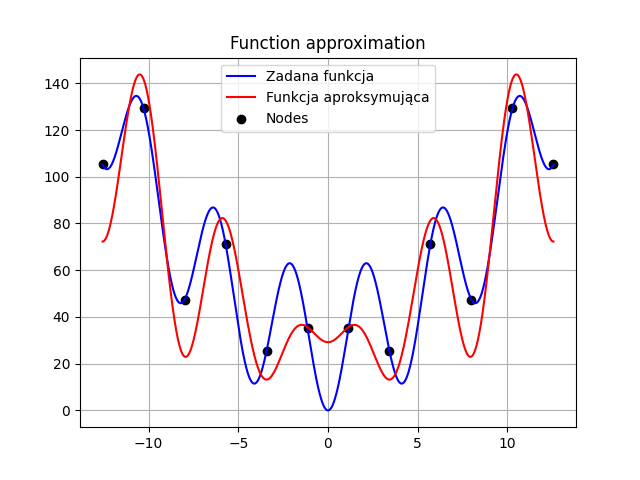
\includegraphics[width=\textwidth]{img34.png}
      \caption{Dla 12 węzłów}
    \end{minipage}
    \vspace*{\fill}
    \begin{minipage}[b]{\textwidth}
      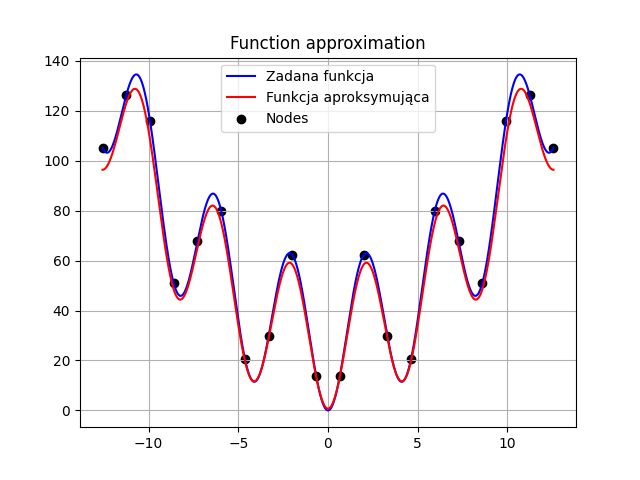
\includegraphics[width=\textwidth]{img35.png}
      \caption{Dla 20 węzłów}
    \end{minipage}
  \end{minipage}
  \hfill
  \begin{minipage}[b]{0.49\textwidth}
    \begin{minipage}[b]{\textwidth}
      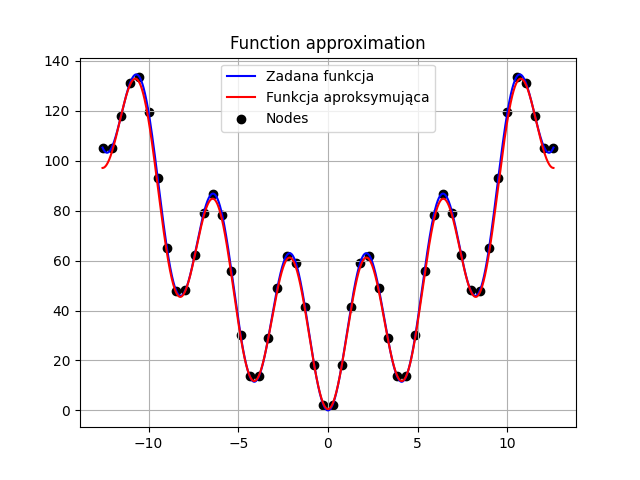
\includegraphics[width=\textwidth]{img36.png}
      \caption{Dla 50 węzłów}
    \end{minipage}
    \vspace*{\fill}
    \begin{minipage}[b]{\textwidth}
      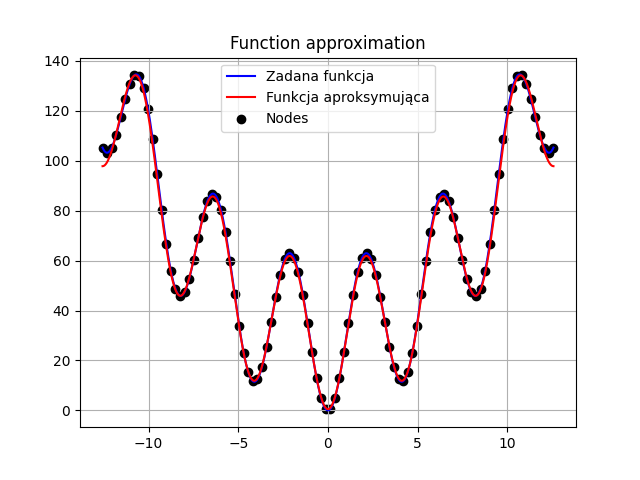
\includegraphics[width=\textwidth]{img37.png}
      \caption{Dla 100 węzłów}
    \end{minipage}
  \end{minipage}
\end{figure}

\noindent
Poniżej, na wykresie 38 przedstawione zostały wartości błędów dla wszystkich możliwych stopni wielomianu.

\begin{figure}[H]
  \centering
  \begin{minipage}[b]{0.4\textwidth}
    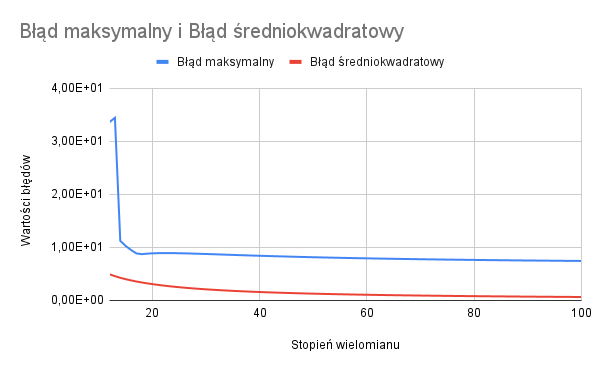
\includegraphics[width=\textwidth]{img38.png}
    \caption{Wartości błędów}
  \end{minipage}
\end{figure}

\newpage

\subsection{Dla 10 stopnia}

\noindent
Jak widać na poniższych wykresach (wykres 39, wykres 40, wykres 41 i wykres 42), przybliżenie jest zdecydowanie lepsze na krańcach przedziałów, niż dla stopnia 6-go.

\begin{figure}[H]
  \begin{minipage}[b]{0.49\textwidth}
    \begin{minipage}[b]{\textwidth}
      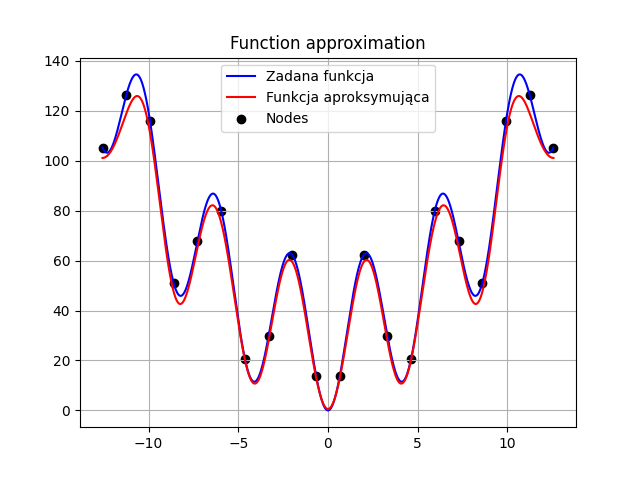
\includegraphics[width=\textwidth]{img39.png}
      \caption{Dla 20 węzłów}
    \end{minipage}
    \vspace*{\fill}
    \begin{minipage}[b]{\textwidth}
      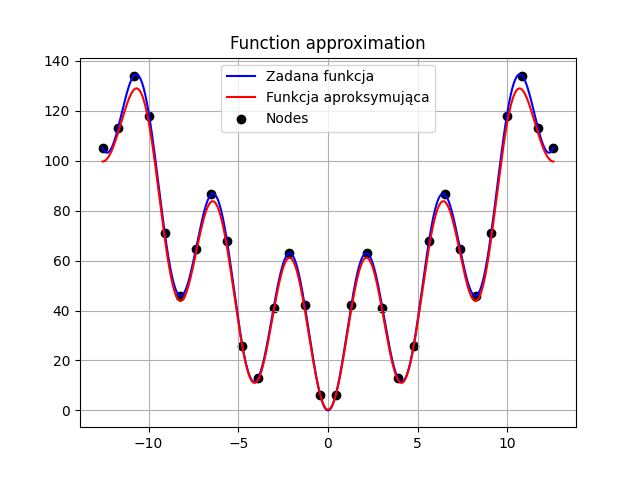
\includegraphics[width=\textwidth]{img40.png}
      \caption{Dla 30 węzłów}
    \end{minipage}
  \end{minipage}
  \hfill
  \begin{minipage}[b]{0.49\textwidth}
    \begin{minipage}[b]{\textwidth}
      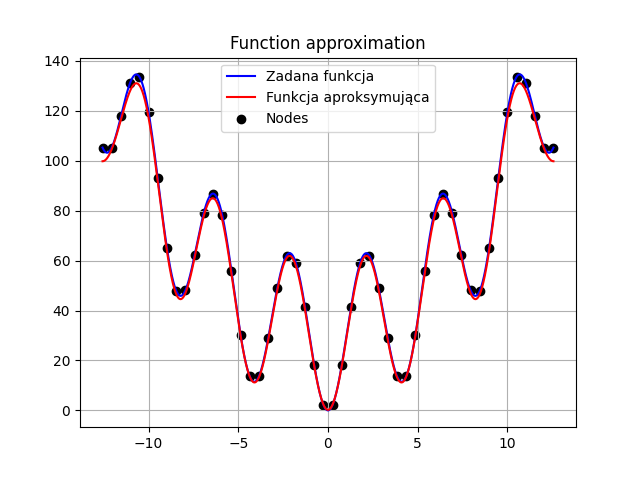
\includegraphics[width=\textwidth]{img41.png}
      \caption{Dla 50 węzłów}
    \end{minipage}
    \vspace*{\fill}
    \begin{minipage}[b]{\textwidth}
      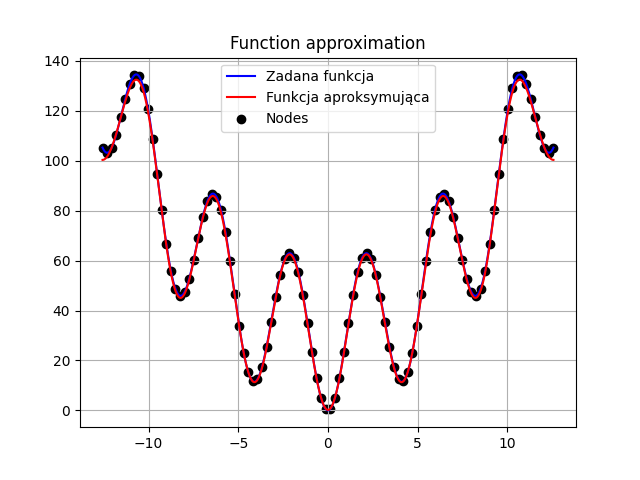
\includegraphics[width=\textwidth]{img42.png}
      \caption{Dla 100 węzłów}
    \end{minipage}
  \end{minipage}
\end{figure}

\noindent
Poniżej, na wykresie 43 przedstawione zostały wartości błędów dla wszystkich możliwych stopni wielomianu.

\begin{figure}[H]
  \centering
  \begin{minipage}[b]{0.4\textwidth}
    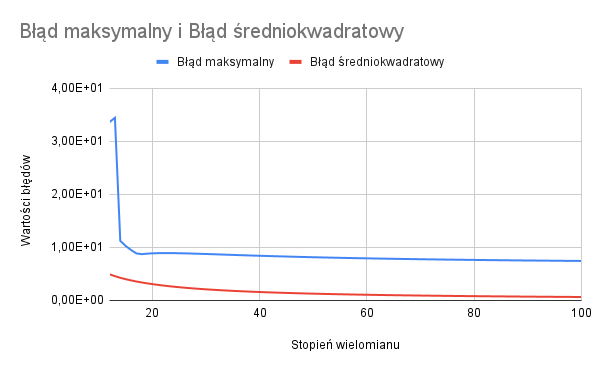
\includegraphics[width=\textwidth]{img43.png}
    \caption{Wartości błędów}
  \end{minipage}
\end{figure}

\newpage

\subsection{Dla 20 stopnia}

\noindent
Dla wielomianu 20-go stopnia przybliżenie na krańcach przedziału staje sie coraz lepsze i błąd jest już niemal niezauważalny (wykres 44, wykres 45, wykres 46 oraz wykres 47).

\begin{figure}[H]
  \begin{minipage}[b]{0.49\textwidth}
    \begin{minipage}[b]{\textwidth}
      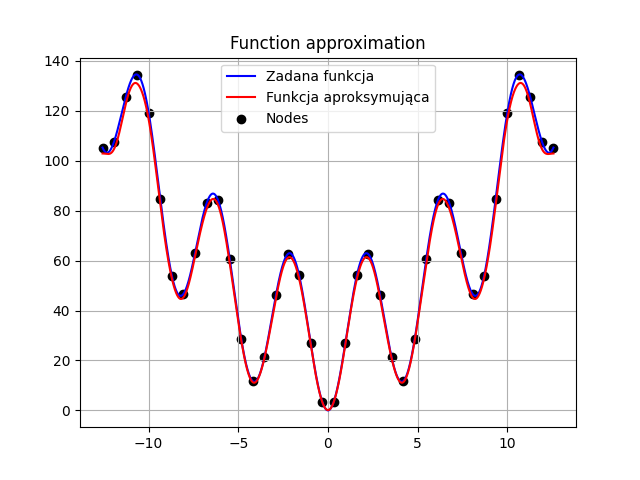
\includegraphics[width=\textwidth]{img44.png}
      \caption{Dla 40 węzłów}
    \end{minipage}
    \vspace*{\fill}
    \begin{minipage}[b]{\textwidth}
      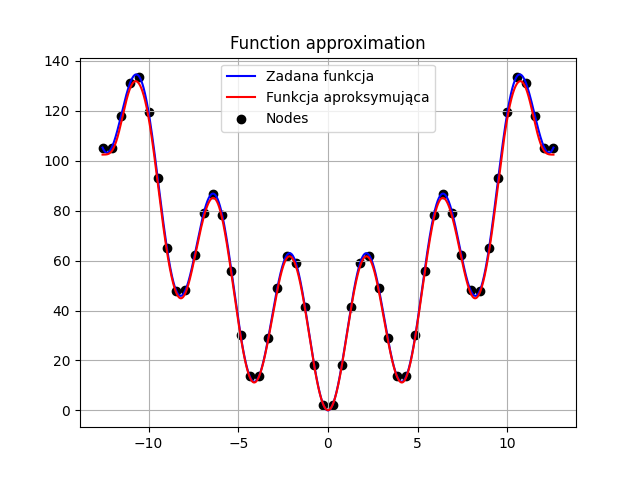
\includegraphics[width=\textwidth]{img45.png}
      \caption{Dla 50 węzłów}
    \end{minipage}
  \end{minipage}
  \hfill
  \begin{minipage}[b]{0.49\textwidth}
    \begin{minipage}[b]{\textwidth}
      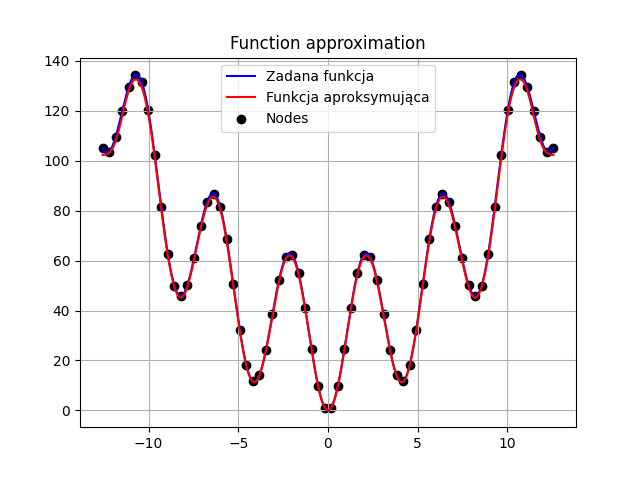
\includegraphics[width=\textwidth]{img46.png}
      \caption{Dla 70 węzłów}
    \end{minipage}
    \vspace*{\fill}
    \begin{minipage}[b]{\textwidth}
      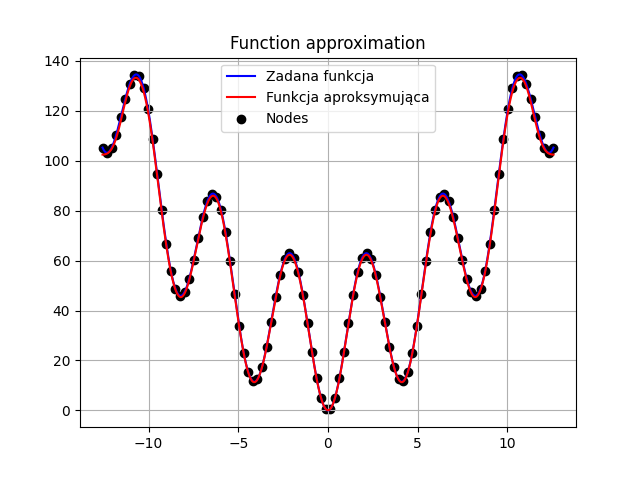
\includegraphics[width=\textwidth]{img47.png}
      \caption{Dla 100 węzłów}
    \end{minipage}
  \end{minipage}
\end{figure}

\noindent
Poniżej, na wykresie 48 przedstawione zostały wartości błędów dla wszystkich możliwych stopni wielomianu.

\begin{figure}[H]
  \centering
  \begin{minipage}[b]{0.4\textwidth}
    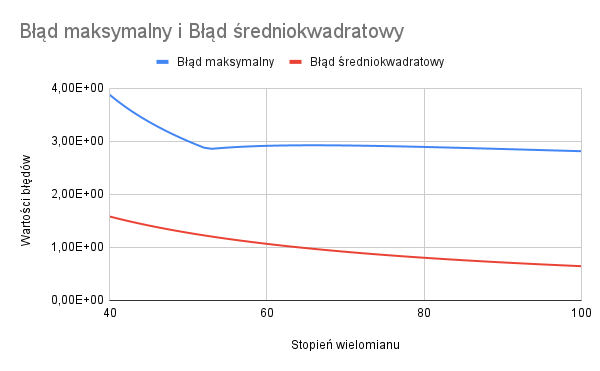
\includegraphics[width=\textwidth]{img48.png}
    \caption{Wartości błędów}
  \end{minipage}
\end{figure}

\newpage

\section{Najlepsze przyblizenie funkcji}

Najlepsze przybliżenie aproksymowanej funkcji otrzymałem dla 50 węzłów i wielomianu 20 stopnia, został on pokazany na poniższym wykresie, a jego błąd maksymalny i średniokwadratowy poniżej w tabelce. Można powiedzieć, że jest to naprawdę dobre przybliżenie.

\begin{figure}[H]
  \centering
  \begin{minipage}[b]{0.4\textwidth}
    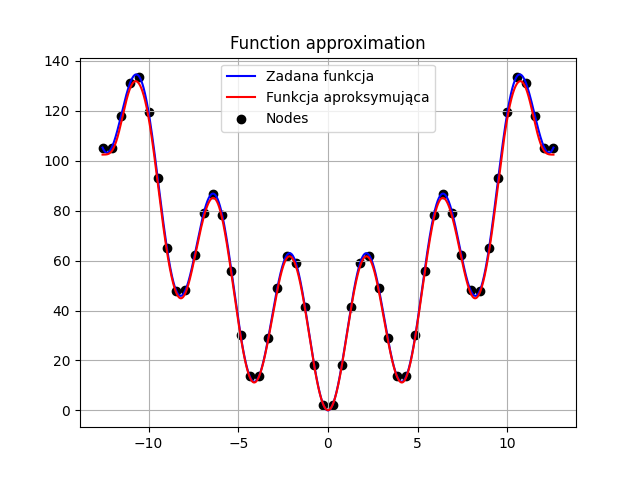
\includegraphics[width=\textwidth]{best.png}
    \caption{Najlepsze przybliżenie funkcji}
  \end{minipage}
\end{figure}

\begin{table}[!ht]
    \centering
    \begin{tabular}{|l|l|}
    \hline
        Błąd maksymalny & 3.001944813353049   \\ \hline
        Błąd średniokwadratowy & 1.2747973802059938 \\ \hline
        
    \end{tabular}
\end{table}

\section{Wnioski}

\begin{itemize}
    \item Aproksymacja wielomianami trygonometrycznimi daje naprawdę dobre przybliżenie funkcji
    \item Od 6 stopnia wielomianu jesteśmy już w stanie otrzymać dobre przybliżenie
    \item Zwiększanie liczby węzłów prowadzi do zwiększenia dokładności przybliżenia
    \item Zwiększanie stopnia wielomianu również powoduje zwiększenie dokładności, ale w dużo mniejszym stopniu.
    \item W tym przypadku układ był dobrze uwarunkowany i jak widać przełożyło się to w znacznym stopniu na otrzymane wyniki.
\end{itemize}

\end{document}
